\chapter{Random Number Generators}
Random Numbers are used in a variety of applications, for example:
\begin{itemize}
  \item simulating random events
  \item professional gaming
  \item end-of-production \& in-field testing of digital systems
  \item Monte Carlo algorithms
  \item cryptographic applications
\end{itemize}
A random number can be generated both via software, or via hardware.\\
Random number are usually needed to generate, in cryptography, some secret data, that is not known 
and unpredictable to an authorized user. To achieve this, the randomization is usually employed.

\begin{boxH}
  A Random Number Generator (RNG) is a utility or device that produces a sequence of numbers 
  within an interval [min, max] while guaranteeing that values appear unpredictable.
\end{boxH}

\begin{subsection}{Characteristics of Random Number generators}
  An RNG should have the following \textbf{3 characteristics}:
  \begin{itemize}
    \item Each new value must be \textbf{statistically independent} of the \textbf{previous value}.
      \subitem That is, given a generated sequence of values, a particular value is not more likely 
       to follow it as the next value in the RNG's random sequence.
    \item The overall distribution of numbers chosen from the interval is \textbf{uniformly distributed}.
      \subitem In other words, all numbers are equally likely, and no one is more “popular” or 
        appears more frequently in the RNG’s output than others.
    \item The sequence is \textbf{unpredictable}
      \subitem An attacker cannot guess some or all the values in a generated sequence. Predictability 
        may take the form of forward prediction (future values) and backtracking (past values).
  \end{itemize}

  In general, the lack of even one of those qualities can introduce severe security vulnerabilities
  that can be exploited by an attacker.\\
  For this reason, the level of care required during the design and implementation of an RNG is
  at least the same required for any other element of a cryptographic system(weakest link principle).
\end{subsection}
\begin{paragraph}{Attack on random numbers}
  Back in the days, some attacks were possible on RNGs, for example the netscape implementation of 
  SSL used a RNG that was predictable, or in Java, it was possible to predict the session ids.\\
  those attacks were possible because the random numbers generated were not unpredictable, being very 
  weak, making it possible to an attackers to break the system.
\end{paragraph}
\begin{section}{True Random Number generators}
  \begin{boxH}
    A \textbf{True Random Number Generator} (TRNG) is an \textbf{hardware primitive} that generates
    random numbers from a physical process, rather than a deterministic algorithm, removing all the
    entropy from the physical world.
  \end{boxH}
  TRNGs are thus often called non-deterministic random number generators since the next number to 
  be generated cannot be determined in advance.\\
  To generate an output that is truly random, a TRNG must rely on a physical process that is
  unpredictable, such as:
  \begin{itemize}
    \item radioactive decay
    \item thermal noise(Johnson-Nyquist noise, or resistor noise)
    \item avalanche noise
    \item timing of keystrokes
    \item audio
  \end{itemize}
  TRNGs, on the other hand, can be quite slow, which is why they are not suitable for all
  applications.
  \begin{paragraph}{Whitening}
    With \textbf{whitening}, we refer to the process of converting a sequence generated by a TRNG
    with the output of a LFSR, to make the output less predictable by increasing the variance.
  \end{paragraph}
  \begin{paragraph}{The most common Analog source}
    The most adopted solutions rely on the following:
    \begin{itemize}
      \item amplifying the noise generated by a resistor (Johnson noise) or by a semiconductor diode
      \item feeding the noise to a comparator or Schmitt trigger
      \item sampling the output of the comparator to get a series of bits that can be used to
        generate random numbers.
    \end{itemize}
  \end{paragraph}
  In some applications, TRNG is implemented simply by measuring internal computer activities that are quantifiable and genuinely random without
  resorting to external custom analog devices.
  \begin{figure}
    \centering
    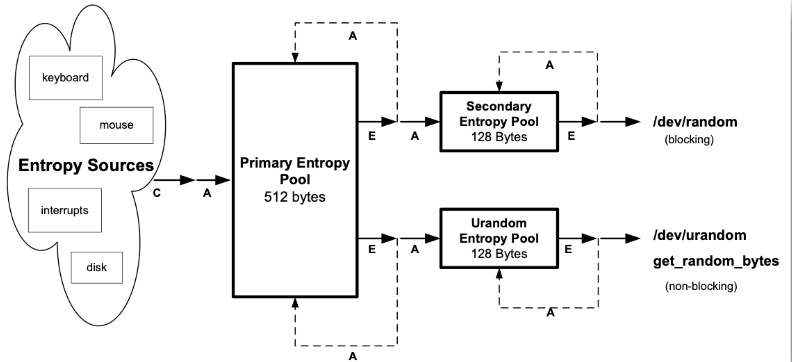
\includegraphics[width=0.5\textwidth]{img/hardware/linux rng.png}
    \caption{the TRNG in the Linux kernel}
  \end{figure}
  To wrap this section up, using system clock, process scheduling, and other system effects may 
  result in some values occurring far more frequently than others:
  \begin{itemize}
    \item When dealing with human-generated entropy, values \textbf{do not distribute evenly} across
      the space of all possible values: some values are more likely to occur than others, and
      certain values rarely occur in practice.
    \item The entropy in the operating system is usually limited, and waiting for more entropy is
      slow and impractical
  \end{itemize}
\end{section}
\begin{section}{Pseudo-Random number generators}
  \begin{boxH}
    A \textbf{Pseudo-Random Number Generator} (PRNG) is an algorithm or a hardware device that
    generates a sequence of random bits (or numbers), starting from an initial value called the
    \textbf{seed}.
  \end{boxH}
  The most common example of this class of RNG is the rand() function in the C standard 
  library.\\
  PNRGS have a characteristic that can be a issue if not properly handled: numbers \textbf{repets periodically}
  and this periodicity depends on the size of the internal state model of the PRNG.
  This is not always a issue for not security related purposes, but mostly this Characteristic can 
  be a dealbreaker for many applications.\\
  The best PRNG algorithms available today have such a large period that this weakness can be 
  practically ignored. For example, the Mersenne Twister MT19937 PRNG with 32-bit word length has a
  periodicity of 219937-1.\\
  Nevertheless, perfect knowledge of the generating circuit and the most recently generated numbers
  could enable one to guess the next number to be generated. For this reason, we test the values to
  know how longer we can stick to the generated sequence before updating it.
  \begin{boxH}
    While a generated sequence of values exhibits the statistical properties
    of randomness (independence, uniform distribution), the overall behaviour of
    the PRNG is entirely predictable.
  \end{boxH}
  For this reason, PRNGs are often called Deterministic random number generators since, given a 
  particular seed value, the same PRNG will always produce the same sequence of “random” numbers.
  \begin{subsection}{Seed criticality}
    To ensure forward unpredictability, care must be taken when obtaining seeds, which should be a 
    true random number.
    After all, the values produced by a PRNG are completely predictable if both the seed and the
    generation algorithm are known.
    Since, in many cases, the generation algorithm is publicly available, the seed
    must be kept secret and generated from a TRNG.
  \end{subsection}
  \begin{subsection}{Hardware PRNG}
    Hardware implementation of a PRNG are mostly made up using \textbf{ALFSR} (Advanced Linear
    Feedback Shift Register), which are basically LFSR which takes no input (but are still able to 
    generate iterate over the whole space of possible values $2^n-1$) and whose characteristic
    polynomial is primitive.
    \begin{figure}[H]
      \centering
      \includegraphics[width=0.5\textwidth]{img/hardware/ALFSR.png}
      \caption{Example of a n-bit ALFSR}
    \end{figure}
    Furthermore, another property of the ALFSR is that if the whole window of amplitude has been
    iterated, each possible value will be generated \textbf{exactly once}, and the sequence will
    repeat.
    \begin{boxH}
      To mask the fact that they are deterministic, PRNGs are often devised to generate more bits
      than needed. For example, a 128-bit ALFSR may be used to implement a 32-bit PRNG.
    \end{boxH}
  \end{subsection}
  \begin{subsection}{Software PRNG}
    Software PRNGs are mostly implemented using programs that implement a recurrence operation.
    One of the most common PRNGs is the \textbf{Linear Congruential Generator} (LCG), which is
    defined by the recurrence relation:
    \begin{equation}
      \begin{cases}
        X_{n+1} = (aX_n + c) \mod m\\
        X_0 = \text{seed}
      \end{cases}
    \end{equation}
    where $a$, $c$, and $m$ are integers, and $X_n$ is the sequence of random numbers generated.
    The normalized sequence of random numbers is given by:
    \begin{equation}
      U_n = \frac{X_n}{M}
    \end{equation}
    where $M$ is usually very large($2^{32}$ or $2^{64}$) because of the modern architectures.\\
    Furthermore, the choice of the parameters $a$, $c$, and $m$ is crucial to the quality of the
    generated sequence. For this purpose the choice involves a sophisticated use of number theory,
    prime numbers and such.
  \end{subsection}

  \begin{subsection}{Cryptographically Secure PRNG}
    PRNGs are considered cryptographically insecure, however, researchers have worked to solve this
    problem by creating what are known as \textbf{Cryptographically Secure PRNGs} (CSPRNGs).\\
    There are \textbf{two} primary \textbf{requirements} for a PRNG to be a CSPRNG:
    \begin{itemize}
    \item Satisfy the next-bit test
      \subitem If someone knows all k bits from the start of the PRNG, they should be unable to predict the bit k+1 using reasonable computing resources.
    \item Withstand the state compromise extensions
      \subitem if an attacker guesses the internal state of the PRNG or it is revealed somehow, they
        should be unable to reconstruct all previous random numbers before the revelation.
    \end{itemize}

    Most CSPRNGs:
    \begin{itemize}
      \item use a combination of entropy from the OS and high-quality PRNG generator
      \item are often “\textbf{reseed}”: when new entropy comes from the OS (e.g., from user input,
        system interruptions, disk I/O or hardware random generators), the underlying PRNG changes
        its internal state based on the new entropy bits coming.
    \end{itemize}
  \end{subsection}

  \begin{subsection}{RNG Conceptual Models}
    One common problem is to generate $K$ random values, which we will call \textit{generated
    values}. We can also assume to have access on a \textit{pool} of $N$ random values, with $N>>K$.
    We can model this problem as the problem to select $K$ random values out of the pool. For this
    reason, an \textbf{extractor} is used, which can either be:
    \begin{itemize}
      \item \textbf{Combinational}: its outputs depend on the current inputs, only
      \item \textbf{Sequential}: its outputs depend on both the current inputs and its internal
        state
    \end{itemize}
    In case of a combinational extractor, the only way to generate sequences of values relies on
    dynamically changing the Pool, for instance, in terms of values, cardinality, sampling time,
    \dots\\
    This peculiar problem can be also modelled in different ways, w.r.t a PRNG:
    \begin{itemize}
      \item the extractor could be modelled as a \textbf{Finite State Machine} (FSM), which iterates
        over the generated values(which are the \textit{states} of the FSM) in a sequential fashion.
      \item the extractor could be modelled as a \textbf{Cryptographic Hash Function}, which has as
        outputs the generated values, or \textit{digests}. This allows the extrator to be both
        constant both combinational.
    \end{itemize}
  \end{subsection}
  \begin{subsection}{Randomness Validation}
    After having generated a random sequence, there's still the need to validate it, to ensure that
    the sequence is actually random.\\
    To this issue, there are plenty of approaches, based on mathematical models and validation
    tests. From a mathematical point of view, the quality of randomness can be measured in bits by
    the \textbf{Shannon Entropy}:
    \begin{equation}
      H(X) = \sum_{x} p(x) \log_2 \frac{1}{p(x)}
    \end{equation}
    which gives us the average amount of information about an elementary event.\\
    Another approach is to simply count that the number of 0s and 1s in the sequence is
    approximately the sane, by breaking down the sequence into blocks of $n$ bits.
    Another approach is to apply \textbf{validation tests} to the generated sequence, for example
    \textit{diagnostic tests} are applied to hort sequences of bits (at least 20.000 bits) to detect
    whether the noise is compromised quickly, which also allow to detect attacks on the RNG. An
    example of this one is the FIPS 140-2 standard.
  \end{subsection}

\end{section}

